\documentclass[11pt]{article}
\usepackage{worksheet_style}

% ---- Toggle: uncomment for filled version ----
%\worksheetfilledtrue
\begin{document}
\worksheetheader{13}{Tangent Planes \& Linear Approximations}

\begin{background}
In Calc I, the tangent line at a point gives the best linear approximation: $f(x) \approx f(a) + f'(a)(x-a)$. Today we extend this to surfaces: the tangent plane is the best flat approximation to $z = f(x,y)$ near a point. This is the foundation of linearization, differentials, and error estimation in multiple dimensions.
\end{background}

%=============================================================
\wsection{From Tangent Lines to Tangent Planes}

-- In Calc I: tangent line at $x = a$ gives $f(x) \approx f(a) + f'(a)(x - a)$

-- In Calc III: the tangent \textit{plane} at $(a,b)$ is the best linear approximation to a surface

\begin{thmbox}{Equation of the Tangent Plane}
The tangent plane to $z = f(x,y)$ at the point $(a, b, f(a,b))$:
\[\boxed{z = \wbml{f(a,b) + f_x(a,b)(x-a) + f_y(a,b)(y-b)}}\]
\end{thmbox}

\begin{center}
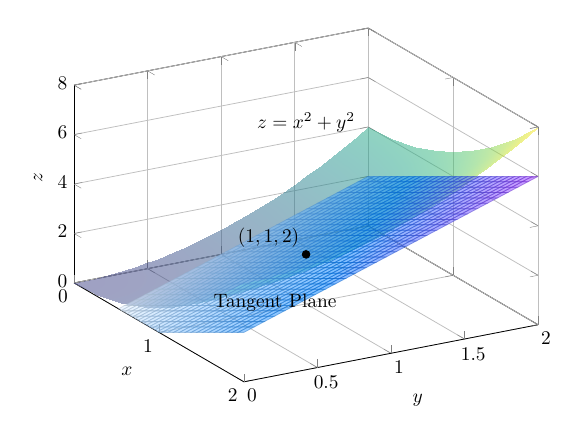
\begin{tikzpicture}[scale=0.7]
  \begin{axis}[
    view={60}{30},
    xlabel={$x$}, ylabel={$y$}, zlabel={$z$},
    domain=-0.5:2.5,
    y domain=-0.5:2.5,
    samples=30,
    samples y=30,
    width=10cm, height=8cm,
    zmin=0, zmax=8,
    grid=major,
    colormap/viridis,
    ztick={0,2,4,6,8}
  ]

    % Plot the surface f(x,y) = x^2 + y^2
    \addplot3[
      surf,
      opacity=0.5,
      shader=interp,
      domain=0:2,
      y domain=0:2,
    ] {x^2 + y^2};

    % Point of tangency (1,1)
    \addplot3[mark=*,color=black] coordinates {(1,1,2)};

    % Compute tangent plane at (1,1):
    % f_x=2x, f_y=2y at (1,1) => f_x=2, f_y=2
    % f(1,1)=1+1=2
    % Tangent plane: z = 2 + 2(x-1) + 2(y-1) = 2x+2y-2
    \addplot3[
      domain=0:2,
      y domain=0:2,
      surf,
      opacity=0.5,
      colormap/cool,
    ] {2*x+2*y-2};

    % Labels
    \node at (axis cs:1,1,2) [anchor=south east] {$(1,1,2)$};
    \node at (axis cs:1,1,8) [anchor=north] {$z=x^2+y^2$};
    \node at (axis cs:1.5,0.5,1) [anchor=south] {Tangent Plane};
  \end{axis}
\end{tikzpicture}
\end{center}

\begin{example}[Tangent Plane to a Paraboloid]
Find the tangent plane to $z = x^2 + y^2$ at $(1, 1, 2)$.

1. \textbf{Compute partials:}

$f_x = 2x$, \quad $f_y = 2y$

2. \textbf{Evaluate at $(1,1)$:}

$f_x(1,1) = $ \wbm{$2$}, \quad $f_y(1,1) = $ \wbm{$2$}, \quad $f(1,1) = $ \wbm{$2$}

3. \textbf{Tangent plane:}

\wbbox{
$z = 2 + 2(x-1) + 2(y-1) = 2 + 2x - 2 + 2y - 2 = \boxed{2x + 2y - 2}$
}{2cm}
\end{example}

\begin{example}[Tangent Plane to $z = y^4 + xy - 2y$ at $(1,1)$]
Find the equation of the tangent plane.

1. \textbf{Function value:} $f(1,1) = 1 + 1 - 2 = $ \wbm{$0$}

2. \textbf{Partials:}

\wbbox{
$f_x = y \implies f_x(1,1) = 1$

$f_y = 4y^3 + x - 2 \implies f_y(1,1) = 4 + 1 - 2 = 3$
}{2cm}

3. \textbf{Result:} $z = 0 + 1(x-1) + 3(y-1) = $ \wbml{$x + 3y - 4$}
\end{example}

%=============================================================
\wsection{Differentiability}

\begin{defbox}{Differentiability in Several Variables}
$f(x,y)$ is \textbf{differentiable} at $(a,b)$ if:
\[f(a+\Delta x, b+\Delta y) = f(a,b) + f_x \Delta x + f_y \Delta y + E(\Delta x, \Delta y)\]
where the error $E$ satisfies $\ds\frac{E}{\sqrt{(\Delta x)^2 + (\Delta y)^2}} \to 0$ as $(\Delta x, \Delta y) \to (0,0)$.

\medskip
-- If $f_x$ and $f_y$ are \textbf{continuous} near $(a,b)$, then $f$ is differentiable there

-- Differentiable $\implies$ continuous (but not the other way around)
\end{defbox}

%=============================================================
\wsection{Linear Approximation}

\begin{formulabox}{Linear Approximation Formula}
\[f(x,y) \approx L(x,y) = \wbml{f(a,b) + f_x(a,b)(x-a) + f_y(a,b)(y-b)}\]
-- The tangent plane \textit{is} the linear approximation

-- Accuracy improves as $(x,y)$ gets closer to $(a,b)$
\end{formulabox}

\begin{example}[Practical Linear Approximation]
Use linear approximation to estimate $f(2.1, 0.9)$ where $f(x,y) = x^2 y - xy^3$.

1. \textbf{Base point:} $(a,b) = (2, 1)$, \; $f(2,1) = 4 - 2 = $ \wbm{$2$}

2. \textbf{Partials at base point:}

\wbbox{
$f_x = 2xy - y^3 \implies f_x(2,1) = 4 - 1 = 3$

$f_y = x^2 - 3xy^2 \implies f_y(2,1) = 4 - 6 = -2$
}{2cm}

3. \textbf{Approximate:}

$L(2.1, 0.9) = 2 + 3(0.1) + (-2)(-0.1) = 2 + 0.3 + 0.2 = $ \wbm{$2.5$}

\medskip
\textit{Check:} $f(2.1, 0.9) = (4.41)(0.9) - (2.1)(0.729) = 3.969 - 1.531 = 2.438$. Error $\approx 0.06$.
\end{example}

%=============================================================
\wsection{Tangent Planes to Implicit Surfaces}

-- For a surface given implicitly as $F(x,y,z) = k$, the gradient $\nabla F$ is normal to the surface

\begin{formulabox}{Tangent Plane to $F(x,y,z) = k$ at $(x_0, y_0, z_0)$}
\[\wbml{F_x(x_0,y_0,z_0)(x-x_0) + F_y(x_0,y_0,z_0)(y-y_0) + F_z(x_0,y_0,z_0)(z-z_0) = 0}\]
Equivalently: $\nabla F \cdot \vec{x-x_0,\; y-y_0,\; z-z_0} = 0$
\end{formulabox}

\begin{example}[Tangent Plane to a Sphere]
Find the tangent plane to $x^2 + y^2 + z^2 = 14$ at $(1, 2, 3)$.

1. \textbf{Set up:} $F(x,y,z) = x^2 + y^2 + z^2$

2. \textbf{Gradient:} $\nabla F = \vec{2x, 2y, 2z}$. At $(1,2,3)$: $\nabla F = $ \wbm{$\vec{2, 4, 6}$}

3. \textbf{Tangent plane:}

\wbbox{
$2(x-1) + 4(y-2) + 6(z-3) = 0$

$2x + 4y + 6z = 28 \implies \boxed{x + 2y + 3z = 14}$
}{2.5cm}
\end{example}

%=============================================================

\begin{practice}

\prob Find the tangent plane to $z = xe^y$ at $(2, 0, 2)$.

\wbbox{
$f_x = e^y \implies f_x(2,0) = 1$. \; $f_y = xe^y \implies f_y(2,0) = 2$.

$z = 2 + 1(x-2) + 2(y-0) = x + 2y$.
}{2.5cm}

\wans{$z = $ \wbml{$x + 2y$}}

\vspace{2.5cm}

\prob Use linear approximation to estimate $\sqrt{(3.02)^2 + (3.97)^2}$.

\textit{Hint:} Let $f(x,y) = \sqrt{x^2+y^2}$ with base point $(3,4)$.

\wbbox{
$f(3,4) = 5$. \; $f_x = x/\sqrt{x^2+y^2} = 3/5$, \; $f_y = y/\sqrt{x^2+y^2} = 4/5$.

$L(3.02, 3.97) = 5 + \frac{3}{5}(0.02) + \frac{4}{5}(-0.03) = 5 + 0.012 - 0.024 = 4.988$.
}{3cm}

\wans{\wbm{$4.988$}}

\vspace{3cm}

\prob Find the tangent plane to $x^2 + 2y^2 + 3z^2 = 36$ at $(1, 2, 3)$.

\wbbox{
$F(x,y,z) = x^2+2y^2+3z^2$. \; $\nabla F = \vec{2x, 4y, 6z}$. At $(1,2,3)$: $\nabla F = \vec{2, 8, 18}$.

$2(x-1) + 8(y-2) + 18(z-3) = 0 \implies x + 4y + 9z = 36$.
}{2.5cm}

\wans{\wbml{$x + 4y + 9z = 36$}}

\vspace{2.5cm}

\prob Find the tangent plane to $z = \sin(xy)$ at $(\pi/2, 1, 1)$ and use it to approximate $f(1.5, 1.1)$.

\wbbox{
$f_x = y\cos(xy) \implies f_x(\pi/2, 1) = \cos(\pi/2) = 0$

$f_y = x\cos(xy) \implies f_y(\pi/2, 1) = \frac{\pi}{2}\cos(\pi/2) = 0$

Tangent plane: $z = 1$. So $f(1.5, 1.1) \approx 1$.

Both partials vanish --- the surface is flat at this peak.
}{3.5cm}

\wans{tangent plane $z = $ \wbm{$1$}, \; $f(1.5, 1.1) \approx$ \wbm{$1$}}

\vspace{3cm}

\prob Two surfaces $z = x^2+y^2$ and $z = 4-x^2-y^2$ intersect along a curve. Find the tangent line to this curve at $(1,1,2)$.

\wbbox{
Tangent plane to $z_1 = x^2+y^2$: $z = 2+2(x-1)+2(y-1)$, i.e., $2x+2y-z=2$.

Tangent plane to $z_2 = 4-x^2-y^2$: $z = 2-2(x-1)-2(y-1)$, i.e., $2x+2y+z=6$.

Tangent line direction: $\vec{2,2,-1}\times\vec{2,2,1} = \vec{4,-4,0} \propto \vec{1,-1,0}$.

Tangent line: $\vect{r}(t) = \vec{1+t, 1-t, 2}$.
}{4.5cm}

\wans{$\vect{r}(t) = $ \wbml{$\vec{1+t,\; 1-t,\; 2}$}}

\end{practice}

\end{document}
